\documentclass[11pt,a4paper]{report}
% ============================================================
%  Shared preamble: colours, typography, boxes, tables, UML/TikZ styles
% ============================================================
\usepackage[T1]{fontenc}
\usepackage[utf8]{inputenc}
\usepackage{mathpazo}
\usepackage[scaled=0.92]{helvet}
\usepackage[a4paper,margin=2.4cm,headheight=15pt]{geometry}
\usepackage[table,dvipsnames]{xcolor}
\usepackage{microtype}
\usepackage{amsmath}
\usepackage{graphicx}
\usepackage{array,booktabs,longtable,tabularx,multirow}
\usepackage{enumitem}
\usepackage{float}
\usepackage[font=small,labelfont={bf,color=navy},textfont=it,skip=6pt]{caption}
\usepackage{fancyhdr}
\usepackage{titlesec}
\usepackage{listings}
\usepackage{tikz}
\usetikzlibrary{arrows.meta,positioning,shapes.geometric,shapes.multipart,shapes.misc,fit,backgrounds,calc,decorations.pathreplacing,patterns}
\usepackage{pgfgantt}
\usepackage[most]{tcolorbox}
\usepackage[colorlinks=true,linkcolor=teal,urlcolor=teal,citecolor=teal]{hyperref}

% ---------- Colour palette ----------
\definecolor{navy}{HTML}{0B2545}
\definecolor{teal}{HTML}{0E8F9C}
\definecolor{tealdark}{HTML}{0A6B75}
\definecolor{amber}{HTML}{F2A33A}
\definecolor{coral}{HTML}{D9534F}
\definecolor{violet}{HTML}{6C4FA1}
\definecolor{leaf}{HTML}{3E9B5F}
\definecolor{mist}{HTML}{EEF3F8}
\definecolor{mint}{HTML}{DDF3F1}
\definecolor{sand}{HTML}{FDF1DC}
\definecolor{blush}{HTML}{FBE3E1}
\definecolor{lilac}{HTML}{E9E3F5}
\definecolor{slate}{HTML}{4A5568}
\definecolor{rowgray}{HTML}{F3F6FA}

% ---------- Project macros (change here only) ----------
\newcommand{\projname}{DocuMind AI}
\newcommand{\projfull}{Intelligent Document Processing and Automated ERP Ingestion System}
\newcommand{\studentname}{Tuheu Tchoubi Pempeme Moussa Fahdil}
\newcommand{\supervisorname}{[Supervisor name -- to be completed]}
\newcommand{\docversion}{2.0}
\newcommand{\docdate}{October 2026}

% ---------- Headings ----------
\titleformat{\chapter}[display]
  {\sffamily\bfseries\color{navy}}
  {\vspace*{-0.5cm}\color{teal}\fontsize{54}{54}\selectfont\thechapter}
  {0.2cm}
  {\Huge}
  [\vspace{2pt}{\color{teal}\titlerule[2.2pt]}]
\titlespacing*{\chapter}{0pt}{0pt}{26pt}
\titleformat{\section}{\sffamily\Large\bfseries\color{navy}}{\color{teal}\thesection}{0.6em}{}
\titleformat{\subsection}{\sffamily\large\bfseries\color{tealdark}}{\thesubsection}{0.6em}{}
\titleformat{\subsubsection}{\sffamily\normalsize\bfseries\color{slate}}{\thesubsubsection}{0.6em}{}
\titlespacing*{\section}{0pt}{16pt}{6pt}
\titlespacing*{\subsection}{0pt}{12pt}{4pt}

% ---------- Header / footer ----------
\pagestyle{fancy}
\fancyhf{}
\renewcommand{\headrulewidth}{0.6pt}
\renewcommand{\headrule}{\hbox to\headwidth{\color{teal}\leaders\hrule height \headrulewidth\hfill}}
\renewcommand{\footrulewidth}{0pt}
\fancyhead[L]{\small\sffamily\color{navy}\projname}
\fancyhead[R]{\small\sffamily\color{slate}\nouppercase{\leftmark}}
\fancyfoot[C]{\small\sffamily\color{slate}\thepage}
\fancypagestyle{plain}{\fancyhf{}\fancyfoot[C]{\small\sffamily\color{slate}\thepage}\renewcommand{\headrulewidth}{0pt}}

% ---------- Lists, spacing ----------
\setlist{itemsep=2pt,topsep=4pt,parsep=0pt}
\setlist[itemize]{label=\textcolor{teal}{\textbullet}}
\setlist[enumerate]{label=\textcolor{teal}{\bfseries\arabic*.}}
\setlength{\parindent}{0pt}
\setlength{\parskip}{6pt}
\renewcommand{\arraystretch}{1.25}
\setcounter{tocdepth}{2}

% ---------- Call-out boxes ----------
\tcbset{calloutbase/.style={enhanced,breakable,sharp corners,boxrule=0pt,leftrule=3.5pt,
  left=8pt,right=8pt,top=6pt,bottom=6pt,fonttitle=\sffamily\bfseries,coltitle=navy,
  attach boxed title to top left={yshift=-2mm},
  boxed title style={colback=white,boxrule=0pt,top=0pt,bottom=0pt,left=0pt}}}
\newtcolorbox{infobox}[1][Note]{calloutbase,colback=mint,colframe=teal,title={#1}}
\newtcolorbox{warnbox}[1][Important]{calloutbase,colback=sand,colframe=amber,title={#1}}
\newtcolorbox{statusbox}[1][Status]{calloutbase,colback=lilac,colframe=violet,title={#1}}
\newtcolorbox{goalbox}[1][Goal]{calloutbase,colback=mist,colframe=navy,title={#1}}

% ---------- Tables ----------
\newcolumntype{L}[1]{>{\raggedright\arraybackslash}p{#1}}
\newcolumntype{C}[1]{>{\centering\arraybackslash}p{#1}}
\newcommand{\hdr}[1]{\textcolor{white}{\sffamily\bfseries #1}}
\newcommand{\tblstart}{\rowcolors{2}{white}{rowgray}\arrayrulecolor{teal!60}}
\newcommand{\hdrrow}{\rowcolor{navy}}
\newcommand{\must}{\textcolor{coral}{\sffamily\bfseries Must}}
\newcommand{\should}{\textcolor{amber!85!black}{\sffamily\bfseries Should}}
\newcommand{\could}{\textcolor{tealdark}{\sffamily\bfseries Could}}
\newcommand{\wont}{\textcolor{slate}{\sffamily\bfseries Won't (now)}}
\newcommand{\done}{\textcolor{leaf}{\sffamily\bfseries Done}}
\newcommand{\inprog}{\textcolor{amber!85!black}{\sffamily\bfseries Partial}}
\newcommand{\todo}{\textcolor{slate}{\sffamily\bfseries Planned}}
\newcommand{\code}[1]{\texttt{\small #1}}

% ---------- Code listings ----------
\lstdefinestyle{docu}{basicstyle=\ttfamily\footnotesize,backgroundcolor=\color{mist},
  frame=l,rulecolor=\color{teal},framerule=3pt,xleftmargin=10pt,framexleftmargin=6pt,
  keywordstyle=\color{tealdark}\bfseries,commentstyle=\color{slate}\itshape,
  stringstyle=\color{violet},showstringspaces=false,breaklines=true,columns=fullflexible,
  aboveskip=8pt,belowskip=8pt}
\lstset{style=docu}

% ---------- TikZ / UML styles ----------
\tikzset{
  every picture/.append style={font=\sffamily\small},
  box/.style={rectangle,rounded corners=3pt,draw=navy,line width=0.7pt,fill=mist,align=center,
              minimum height=0.8cm,inner sep=4pt},
  boxT/.style={box,fill=mint,draw=tealdark},
  boxA/.style={box,fill=sand,draw=amber!80!black},
  boxV/.style={box,fill=lilac,draw=violet},
  boxC/.style={box,fill=blush,draw=coral},
  boxN/.style={box,fill=navy,draw=navy,text=white},
  arr/.style={-{Stealth[length=2.6mm,width=1.9mm]},line width=0.7pt,color=navy},
  arrd/.style={-{Stealth[length=2.6mm,width=1.9mm]},line width=0.7pt,color=slate,dashed},
  lbl/.style={font=\sffamily\scriptsize,color=slate,fill=white,inner sep=1.2pt},
  state/.style={rectangle,rounded corners=8pt,draw=tealdark,fill=mint,line width=0.8pt,
                minimum width=2.5cm,minimum height=0.9cm,align=center,font=\sffamily\footnotesize\bfseries},
  stateA/.style={state,fill=sand,draw=amber!80!black},
  stateC/.style={state,fill=blush,draw=coral},
  stateV/.style={state,fill=lilac,draw=violet},
  initial/.style={circle,fill=navy,minimum size=0.35cm,inner sep=0pt},
  final/.style={circle,draw=navy,line width=0.9pt,minimum size=0.5cm,inner sep=0pt,
                path picture={\fill[navy] (path picture bounding box.center) circle (0.17cm);}},
  uclass/.style={rectangle split,rectangle split parts=3,draw=navy,line width=0.8pt,fill=white,
                 font=\sffamily\scriptsize,text width=3.55cm,inner sep=3pt,align=left,
                 rectangle split part fill={mint,white,white}},
  uclass2/.style={rectangle split,rectangle split parts=2,draw=navy,line width=0.8pt,fill=white,
                 font=\sffamily\scriptsize,text width=3.55cm,inner sep=3pt,align=left,
                 rectangle split part fill={mint,white}},
  uiface/.style={uclass2,rectangle split part fill={sand,white}},
  uenum/.style={uclass2,rectangle split part fill={lilac,white}},
  ucase/.style={ellipse,draw=tealdark,fill=mint,line width=0.7pt,align=center,
                font=\sffamily\scriptsize,minimum height=0.8cm,inner xsep=3pt},
  lifeline/.style={dashed,color=slate,line width=0.6pt},
  msg/.style={-{Stealth[length=2.4mm,width=1.7mm]},line width=0.65pt,color=navy},
  ret/.style={-{Stealth[length=2.4mm,width=1.7mm]},line width=0.65pt,color=slate,dashed},
}
% stick-figure actor: \actor{name}{x}{y}{label}
\newcommand{\actor}[4]{%
  \begin{scope}[shift={(#2,#3)},color=navy,line width=0.9pt]
    \draw[fill=sand] (0,0.95) circle (0.2);
    \draw (0,0.75)--(0,0.1) (-0.35,0.55)--(0.35,0.55) (0,0.1)--(-0.28,-0.4) (0,0.1)--(0.28,-0.4);
    \node[font=\sffamily\scriptsize\bfseries,text=navy,align=center,below] (#1) at (0,-0.38) {#4};
  \end{scope}}
% class-name helper (centred bold)
\newcommand{\cname}[1]{\centerline{\bfseries #1}}
\newcommand{\stereo}[1]{\guillemotleft\,#1\,\guillemotright}

\hypersetup{pdftitle={DocuMind AI - Phase 1 Requirements Specification},pdfauthor={Tuheu Tchoubi Pempeme Moussa Fahdil}}
\begin{document}
\begin{titlepage}
\newgeometry{margin=0cm}
\thispagestyle{empty}
\begin{tikzpicture}[remember picture,overlay]
  \fill[navy] (current page.north west) rectangle ([yshift=-17.5cm]current page.north east);
  \fill[teal] ([yshift=-17.5cm]current page.north west) rectangle ([yshift=-17.9cm]current page.north east);
  \fill[amber] ([yshift=-17.9cm]current page.north west) rectangle ([yshift=-18.1cm]current page.north east);
  % decorative document / network motif
  \begin{scope}[shift={([xshift=-8.2cm,yshift=-4.6cm]current page.north east)},opacity=0.9]
    \draw[teal!70,line width=1pt,fill=white!8!navy] (0,0) rectangle (2.6,3.4);
    \foreach \y in {0.5,0.9,1.3,1.7,2.1} {\draw[teal!70,line width=0.8pt] (0.3,\y) -- (2.3,\y);}
    \draw[amber,line width=1.4pt,fill=amber!25!navy] (0.3,2.5) rectangle (1.5,2.9);
    \draw[-{Stealth},amber,line width=1.2pt] (2.8,1.7) -- (4.0,1.7);
    \draw[teal!70,line width=1pt,fill=white!8!navy] (4.2,0.9) rectangle (5.3,2.5);
    \foreach \y in {1.2,1.6,2.0} {\draw[teal!70,line width=0.8pt] (4.4,\y) -- (5.1,\y);}
  \end{scope}
  \node[anchor=west,text=white,font=\sffamily\bfseries\fontsize{40}{44}\selectfont] at ([xshift=2.4cm,yshift=-9.3cm]current page.north west) {\projname};
  \node[anchor=west,text=teal!30,font=\sffamily\fontsize{15}{19}\selectfont,text width=15cm] at ([xshift=2.4cm,yshift=-11.5cm]current page.north west) {Intelligent Document Processing and\\ Automated ERP Ingestion System};
  \node[anchor=west,text=white,font=\sffamily\small,text width=15cm] at ([xshift=2.4cm,yshift=-13.7cm]current page.north west) {Phase 1 -- Requirements Analysis and Planning};
  \node[anchor=west,text=amber,font=\sffamily\bfseries\footnotesize] at ([xshift=2.4cm,yshift=-15.3cm]current page.north west) {REQUIREMENTS SPECIFICATION \ $\cdot$ \ SCOPE \ $\cdot$ \ RISKS \ $\cdot$ \ PROJECT PLAN};
  \node[anchor=west,text=white!70,font=\sffamily\scriptsize] at ([xshift=2.4cm,yshift=-3.0cm]current page.north west) {ICT UNIVERSITY \ $\cdot$ \ FACULTY OF ICT \ $\cdot$ \ DEPARTMENT OF COMPUTER SCIENCE};
\end{tikzpicture}
\begin{tikzpicture}[remember picture,overlay]
\node[anchor=north west,text width=15.5cm,font=\sffamily\small] at ([xshift=2.4cm,yshift=-19.3cm]current page.north west) {%
\begin{tabular}{@{}L{3.2cm}L{11cm}@{}}
\textcolor{teal}{\bfseries Student}   & \studentname\\
\textcolor{teal}{\bfseries Programme} & B.Sc. Computer Science, final-year project\\
\textcolor{teal}{\bfseries Supervisor}& \supervisorname\\
\textcolor{teal}{\bfseries Institution}& The ICT University, Cameroon\\
\textcolor{teal}{\bfseries Version}    & \docversion \ -- \docdate\\
\end{tabular}};
\end{tikzpicture}
\restoregeometry
\end{titlepage}

\pagenumbering{roman}
\chapter*{Document Control}
\addcontentsline{toc}{chapter}{Document Control}
\tblstart\small
\begin{longtable}{L{3.4cm}L{11.0cm}}
\hdrrow \hdr{Item} & \hdr{Description}\\ \endhead
Document & \projname{} -- Phase 1: Requirements Analysis and Planning.\\
Version & \docversion{} (\docdate).\\
Deliverable & Requirements specification: problem analysis, objectives, scope, stakeholders, functional and non-functional requirements, use cases, data requirements, success metrics, risks, project plan and traceability.\\
Related document & \emph{Project Design Document} (architecture, UML, data and API design).\\
Status & \textbf{Draft for supervisor review.} Items marked \emph{[Decision needed]} must be confirmed before Phase 1 is closed (Section~\ref{sec:decisions}).\\
Honesty note & Targets in this document are planning values. No result is claimed.\\
\hline
\end{longtable}
\clearpage
\tableofcontents
\clearpage
\listoffigures
\clearpage
\pagenumbering{arabic}
\setcounter{page}{1}

\chapter{Purpose and Summary}
\section{Purpose of this document}
Phase 1 answers four questions before any serious development starts: \emph{what problem are we solving, for whom, within which limits, and how will we know we succeeded?} The answers are written as testable requirements so that design (Phase 2), implementation and evaluation can all be traced back to them.

\section{Project in one paragraph}
\projname{} receives supplier invoices (PDF, PNG or JPEG) in French or English, improves image quality, recognises the text with a custom-trained OCR model compared against an established baseline, extracts the key invoice fields, validates them with business rules, asks a human reviewer to confirm uncertain values, and finally sends approved records to an ERP system (a mock or sandbox first, Odoo as target) with a complete audit trail.

\section{Phase 1 at a glance}
{\tblstart\small
\begin{longtable}{L{4.0cm}L{9.8cm}}
\hdrrow \hdr{Topic} & \hdr{Position taken in this document}\\ \endhead
Document type & Invoices only for the prototype; other documents are later extensions.\\
Languages & French and English.\\
Input formats & PDF, PNG, JPEG.\\
Human review & Mandatory before any ERP submission.\\
ERP target & Mock ERP first; Odoo when access and version are confirmed.\\
OCR & Custom CRNN + CTC model, evaluated honestly against Tesseract.\\
Architecture & Modular monolith first, then Docker Compose, then services and Kubernetes.\\
Requirements & 22 functional and 10 non-functional requirements with acceptance criteria.\\
\hline
\end{longtable}}

\chapter{Problem Analysis}
\section{Current situation (as-is)}
Invoices arrive by e-mail, on paper or as scans. An employee reads each one and types the values into the ERP by hand, usually without a systematic check and without a record of who changed what.

\begin{figure}[H]\centering
\resizebox{\textwidth}{!}{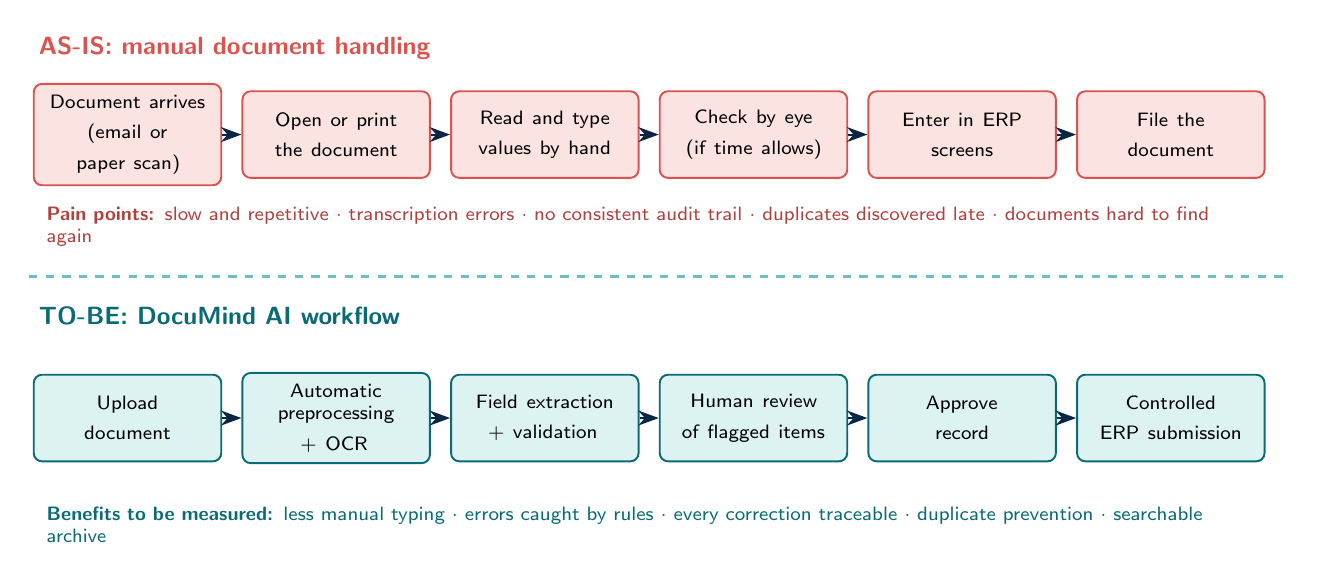
\begin{tikzpicture}[x=1cm,y=1cm]
\node[font=\sffamily\bfseries\small,text=coral,anchor=west] at (0,5.6) {AS-IS: manual document handling};
\foreach \i/\t in {0/Document arrives\\ (email or paper scan),1/Open or print\\ the document,2/Read and type\\ values by hand,3/Check by eye\\ (if time allows),4/Enter in ERP\\ screens,5/File the\\ document}{
  \node[boxC,text width=2.1cm,minimum height=1.1cm] (a\i) at (1.25+2.65*\i,4.5) {\scriptsize\t};}
\foreach \i/\j in {0/1,1/2,2/3,3/4,4/5}{\draw[arr] (a\i) -- (a\j);}
\node[font=\sffamily\scriptsize,text=coral!80!black,text width=15cm,align=left,anchor=north west] at (0.1,3.7) {\textbf{Pain points:} slow and repetitive $\cdot$ transcription errors $\cdot$ no consistent audit trail $\cdot$ duplicates discovered late $\cdot$ documents hard to find again};
\draw[teal!60,line width=1pt,dashed] (0,2.7) -- (16,2.7);
\node[font=\sffamily\bfseries\small,text=tealdark,anchor=west] at (0,2.2) {TO-BE: \projname{} workflow};
\foreach \i/\t in {0/Upload\\ document,1/Automatic\\ preprocessing\\ + OCR,2/Field extraction\\ + validation,3/Human review\\ of flagged items,4/Approve\\ record,5/Controlled\\ ERP submission}{
  \node[boxT,text width=2.1cm,minimum height=1.1cm] (b\i) at (1.25+2.65*\i,0.9) {\scriptsize\t};}
\foreach \i/\j in {0/1,1/2,2/3,3/4,4/5}{\draw[arr] (b\i) -- (b\j);}
\node[font=\sffamily\scriptsize,text=tealdark,text width=15cm,align=left,anchor=north west] at (0.1,-0.1) {\textbf{Benefits to be measured:} less manual typing $\cdot$ errors caught by rules $\cdot$ every correction traceable $\cdot$ duplicate prevention $\cdot$ searchable archive};
\end{tikzpicture}
}
\caption{Manual process (as-is) compared with the proposed workflow (to-be).}\label{fig:asis}
\end{figure}

\section{Problems identified}
{\tblstart\small
\begin{longtable}{L{1.0cm}L{4.0cm}L{8.7cm}}
\hdrrow \hdr{ID} & \hdr{Problem} & \hdr{Consequence}\\ \endhead
P1 & Manual re-typing & Slow, repetitive work that does not scale with volume.\\
P2 & Transcription errors & Wrong amounts, dates or supplier data enter the ERP.\\
P3 & No systematic validation & Totals that do not match subtotal plus tax go unnoticed.\\
P4 & Duplicate invoices & The same invoice may be paid twice.\\
P5 & No audit trail & Corrections cannot be traced to a person or a reason.\\
P6 & Documents hard to retrieve & Originals are scattered across mailboxes and folders.\\
\hline
\end{longtable}}

\section{Proposed solution (to-be)}
Automate the repetitive steps (reading, extracting, cross-checking) and keep the human where judgement matters (resolving uncertainty, approving). Every document and every correction is stored with identifiers and timestamps.

\section{System context}
\begin{figure}[H]\centering
\resizebox{0.95\textwidth}{!}{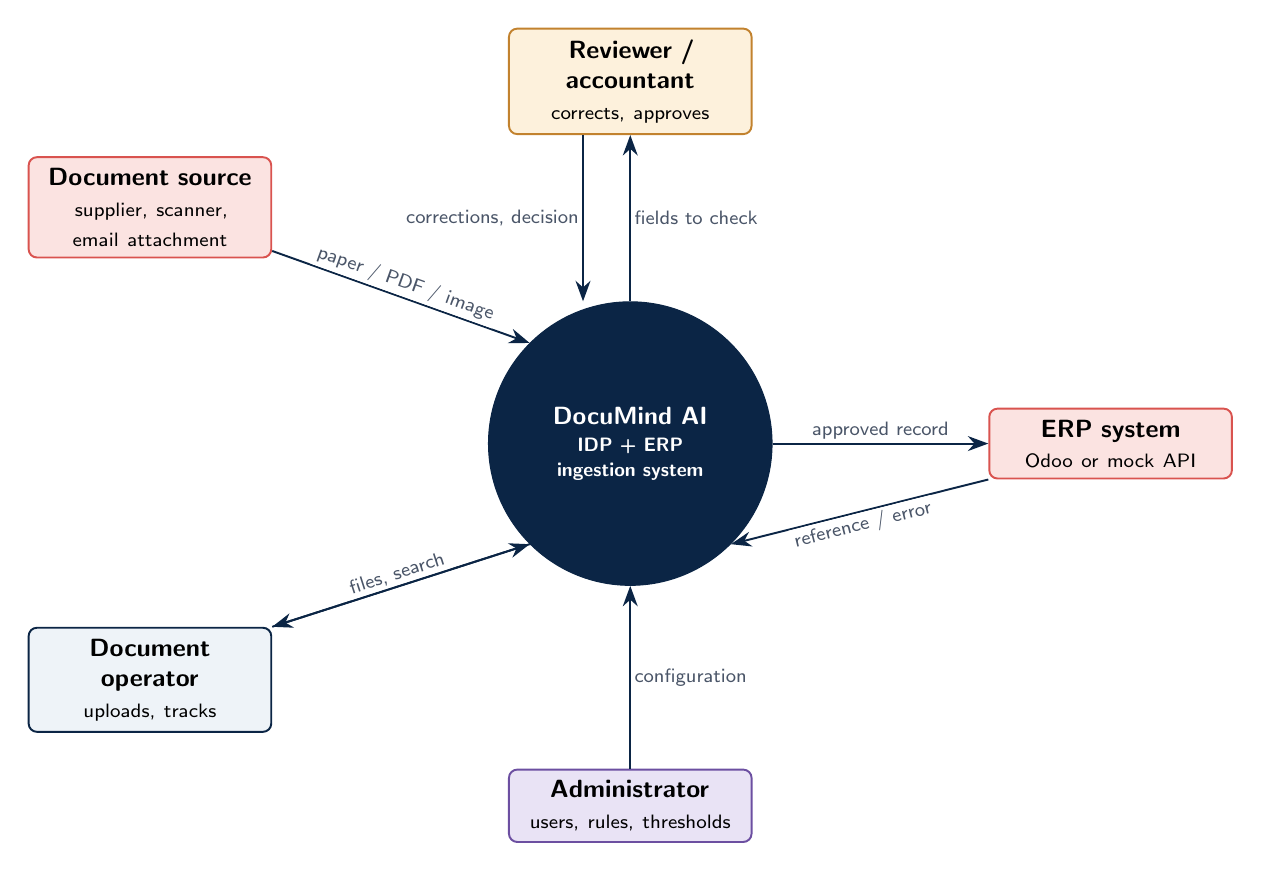
\begin{tikzpicture}[x=1cm,y=1cm]
\node[circle,draw=navy,fill=navy,text=white,font=\sffamily\bfseries\small,align=center,minimum size=3.6cm] (sys) at (8,4) {\projname\\[-1pt]\scriptsize IDP + ERP\\[-2pt]\scriptsize ingestion system};
\node[boxC,minimum width=3cm,text width=2.8cm] (src) at (1.9,7.0) {\textbf{Document source}\\\scriptsize supplier, scanner, email attachment};
\node[box,minimum width=3cm,text width=2.8cm] (op) at (1.9,1.0) {\textbf{Document operator}\\\scriptsize uploads, tracks};
\node[boxA,minimum width=3cm,text width=2.8cm] (rv) at (8,8.6) {\textbf{Reviewer / accountant}\\\scriptsize corrects, approves};
\node[boxV,minimum width=3cm,text width=2.8cm] (ad) at (8,-0.6) {\textbf{Administrator}\\\scriptsize users, rules, thresholds};
\node[boxC,minimum width=3cm,text width=2.8cm,fill=blush] (erp) at (14.1,4.0) {\textbf{ERP system}\\\scriptsize Odoo or mock API};
\draw[arr] (src) -- node[lbl,sloped,above]{paper / PDF / image} (sys.north west);
\draw[arr] (op.north east) -- node[lbl,sloped,above]{files, search} (sys.south west);
\draw[arr] (sys.south west) -- (op.north east);
\draw[arr] (sys.north) -- node[lbl,right]{fields to check} (rv.south);
\draw[arr] ([xshift=-6mm]rv.south) -- node[lbl,left]{corrections, decision} ([xshift=-6mm]sys.north |- sys.north);
\draw[arr] (ad.north) -- node[lbl,right]{configuration} (sys.south);
\draw[arr] (sys.east) -- node[lbl,above]{approved record} (erp.west);
\draw[arr] (erp.south west) -- node[lbl,sloped,below]{reference / error} (sys.south east);
\end{tikzpicture}
}
\caption{Context diagram: the system, its users and external systems.}\label{fig:context}
\end{figure}

\chapter{Objectives and Success Criteria}
\section{Aim}
To design and implement a secure, modular system that extracts structured information from French and English invoices and prepares validated records for ERP ingestion.

\section{Objectives with measurable success criteria}
{\tblstart\small
\begin{longtable}{L{1.0cm}L{5.4cm}L{7.3cm}}
\hdrrow \hdr{ID} & \hdr{Objective} & \hdr{Success criterion (to be verified in Phase 14)}\\ \endhead
O1 & Secure upload and lifecycle tracking & A valid invoice receives an ID and persistent status; invalid files are refused with a clear reason.\\
O2 & Improve scan readability & Preprocessing reduces CER on the test set versus no preprocessing (reported, not assumed).\\
O3 & Custom OCR for French and English & CER and WER reported on a held-out set alongside the Tesseract baseline.\\
O4 & Extract key invoice fields & Per-field precision, recall and F1 reported for the field list in Section~\ref{sec:fields}.\\
O5 & Confidence and review routing & Flagged records and their error rates reported; thresholds chosen on validation data only.\\
O6 & Validate extracted data & Seeded error cases (wrong total, bad date, duplicate) are detected in tests.\\
O7 & Review dashboard & A reviewer completes correct-and-approve tasks in a usability check.\\
O8 & Persist data and audit trail & Every correction, approval and ERP attempt appears in the audit log.\\
O9 & ERP integration & Mock/sandbox demonstrates success, failure and retry with zero duplicate records.\\
O10 & Containerised delivery & A new machine runs the system from the documented setup in a clean environment.\\
\hline
\end{longtable}}

\section{Provisional quantitative targets}
\label{sec:targets}
\begin{warnbox}[Planning values, not results]
The numbers below only give the experiments a goal. They will be revised after the baseline measurement (Phase 7) and must never be quoted in the report as achieved results.
\end{warnbox}
{\tblstart\small
\begin{longtable}{L{4.6cm}L{4.4cm}L{4.8cm}}
\hdrrow \hdr{Metric} & \hdr{Provisional target} & \hdr{Revision point}\\ \endhead
CER / WER (custom model) & Compete with the Tesseract baseline on the same test set & Absolute target set after Phase 7\\
Field F1: invoice number, date, total & $\geq 0.85$ before human review & After Phase 9 first run\\
Arithmetic-error detection & All seeded error cases detected & Phase 10\\
Duplicate ERP submissions & 0 in retry tests & Phase 12\\
Median time per single-page invoice & Reported (no fixed target) & After Phase 7\\
Upload rejection of invalid files & 100\% of defined invalid test files & Phase 5\\
\hline
\end{longtable}}

\chapter{Scope}
\section{In scope (first prototype)}
\begin{itemize}
\item Supplier invoices as PDF, PNG or JPEG, French and English, printed or cleanly scanned.
\item Preprocessing, OCR (custom and baseline), extraction, validation, confidence scoring.
\item Human review with correction, approval, rejection and audit trail.
\item ERP adapter with a mock or sandbox ERP; Odoo mapping documented.
\item React web dashboard, FastAPI backend, MySQL, Docker.
\end{itemize}

\section{Out of scope}
\begin{itemize}
\item Handwritten invoices and very low-quality photographs.
\item Other document types (purchase orders, receipts, forms) -- listed as future work.
\item Fully automatic posting without human approval.
\item Production ERP connection and any claim of legal or accounting compliance.
\item Mobile application and offline mode.
\end{itemize}

\section{Supported document types: decision}
{\tblstart\small
\begin{longtable}{L{3.4cm}L{2.6cm}L{7.8cm}}
\hdrrow \hdr{Document type} & \hdr{Prototype?} & \hdr{Reason}\\ \endhead
Invoice & \textbf{Yes} & Clear field set, directly useful for ERP ingestion, arithmetic gives strong validation rules.\\
Purchase order & Later & Similar fields; add after the invoice workflow works.\\
Receipt & Later & Variable layouts and thermal-print quality make OCR harder.\\
Administrative form & Later & Needs form-specific templates.\\
\hline
\end{longtable}}

\chapter{Stakeholders and Users}
\section{Stakeholder analysis}
\begin{figure}[H]\centering
\resizebox{0.62\textwidth}{!}{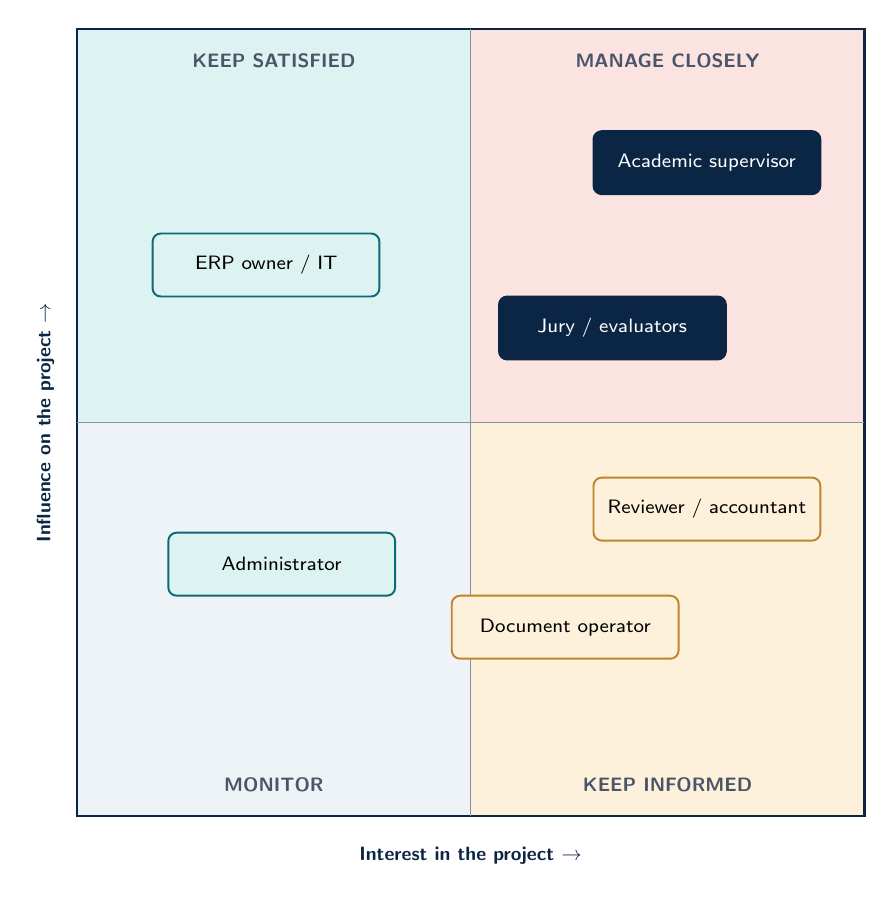
\begin{tikzpicture}[x=1cm,y=1cm]
\fill[mist]  (0,0) rectangle (5,5);   \fill[sand] (5,0) rectangle (10,5);
\fill[mint]  (0,5) rectangle (5,10);  \fill[blush] (5,5) rectangle (10,10);
\draw[navy,line width=0.8pt] (0,0) rectangle (10,10); \draw[navy!50] (5,0) -- (5,10) (0,5) -- (10,5);
\node[font=\sffamily\scriptsize\bfseries,text=slate] at (2.5,9.6) {KEEP SATISFIED};
\node[font=\sffamily\scriptsize\bfseries,text=slate] at (7.5,9.6) {MANAGE CLOSELY};
\node[font=\sffamily\scriptsize\bfseries,text=slate] at (2.5,0.4) {MONITOR};
\node[font=\sffamily\scriptsize\bfseries,text=slate] at (7.5,0.4) {KEEP INFORMED};
\node[boxN,text width=2.6cm,font=\sffamily\scriptsize] at (8.0,8.3) {Academic supervisor};
\node[boxN,text width=2.6cm,font=\sffamily\scriptsize] at (6.8,6.2) {Jury / evaluators};
\node[boxA,text width=2.6cm,font=\sffamily\scriptsize] at (8.0,3.9) {Reviewer / accountant};
\node[boxA,text width=2.6cm,font=\sffamily\scriptsize] at (6.2,2.4) {Document operator};
\node[boxT,text width=2.6cm,font=\sffamily\scriptsize] at (2.4,7.0) {ERP owner / IT};
\node[boxT,text width=2.6cm,font=\sffamily\scriptsize] at (2.6,3.2) {Administrator};
\node[rotate=90,font=\sffamily\scriptsize\bfseries,text=navy] at (-0.4,5) {Influence on the project $\rightarrow$};
\node[font=\sffamily\scriptsize\bfseries,text=navy] at (5,-0.5) {Interest in the project $\rightarrow$};
\end{tikzpicture}
}
\caption{Influence--interest grid (initial judgement; adjust with the supervisor).}\label{fig:stake}
\end{figure}

{\tblstart\small
\begin{longtable}{L{3.2cm}L{5.4cm}L{5.2cm}}
\hdrrow \hdr{Stakeholder} & \hdr{Needs} & \hdr{Involvement}\\ \endhead
Academic supervisor & Rigour, honest evaluation, progress evidence. & Reviews documents and milestones.\\
Jury / evaluators & Clear architecture, working demonstration, measured results. & Final defence.\\
Reviewer / accountant & Fast, trustworthy correction of uncertain fields. & Main interactive user of the review screen.\\
Document operator & Simple upload and status tracking. & Daily user.\\
Administrator & Control of users, rules and thresholds. & Configuration and oversight.\\
ERP owner / IT & Clean, safe, non-duplicating integration. & Provides interface details (open decision).\\
\hline
\end{longtable}}

\section{User roles}
Four roles are enforced by the backend: \textbf{Administrator}, \textbf{Operator}, \textbf{Reviewer} and \textbf{Integration service account}. A supervisor or auditor receives read-only access to logs and metrics.

\section{User stories}
{\tblstart\small
\begin{longtable}{L{1.2cm}L{10.4cm}L{2.0cm}}
\hdrrow \hdr{ID} & \hdr{Story} & \hdr{Req.}\\ \endhead
US-01 & As an operator, I upload an invoice and immediately get an ID and status, so that I know it was received. & FR-03, 05, 06\\
US-02 & As an operator, I see why a bad file was refused, so that I can send a correct one. & FR-04\\
US-03 & As a reviewer, I see the source page next to the extracted fields with doubtful values highlighted, so that I check only what matters. & FR-11, 22\\
US-04 & As a reviewer, I correct a value and give a reason, so that the change is traceable. & FR-12, 13\\
US-05 & As a reviewer, I approve or reject a record, so that only checked data reaches the ERP. & FR-12, 14\\
US-06 & As an administrator, I adjust review thresholds and validation rules without changing code. & FR-17\\
US-07 & As an accountant, I am warned about a probable duplicate invoice before it is posted. & FR-10, 11\\
US-08 & As an auditor, I see who changed what and when. & FR-13\\
US-09 & As an operator, I resubmit a failed document for processing. & FR-21\\
US-10 & As the ERP owner, I need a failed submission to be retryable without creating a second record. & FR-15\\
\hline
\end{longtable}}

\chapter{Functional Requirements}
\section{Requirement list with acceptance criteria}
Priorities follow MoSCoW: \must{} (needed for the prototype), \should{} (important, can slip), \could{} (nice to have). Each requirement has an acceptance criterion that becomes a test in Phase 14.

{\tblstart\footnotesize
\begin{longtable}{L{1.2cm}L{5.6cm}L{1.3cm}L{5.4cm}}
\hdrrow \hdr{ID} & \hdr{Requirement} & \hdr{Prio.} & \hdr{Acceptance criterion}\\ \endhead
FR-01 & A permitted user can sign in and sign out. & \must & Valid credentials give access; invalid ones are refused; logout invalidates the session.\\
FR-02 & Role-based access to admin, operational and review functions. & \must & Each role can call only its endpoints; others return 403.\\
FR-03 & Upload PDF, PNG or JPEG within configured limits. & \must & Valid file returns a document ID.\\
FR-04 & Check file type, size and basic integrity. & \must & Oversized, wrong-type and corrupt files are refused (413/415/400).\\
FR-05 & Store the original privately with a unique ID and SHA-256. & \must & File is not reachable without authorisation; hash stored.\\
FR-06 & Create a processing job with status and timestamps. & \must & Status and times visible after upload.\\
FR-07 & Normalise pages and enhance images. & \must & Pages are rendered and preprocessed; intermediates retrievable in debug mode.\\
FR-08 & OCR returns text and confidence where supported. & \must & Output contains text per line with a confidence value.\\
FR-09 & Map recognised content to configured invoice fields. & \must & Field list in Section~\ref{sec:fields} produced for a test invoice.\\
FR-10 & Validate required fields, formats, arithmetic and duplicates. & \must & Seeded invalid invoices raise the expected findings.\\
FR-11 & Flag low-confidence or invalid records for review. & \must & Flagged records enter the review queue.\\
FR-12 & Reviewer can correct, give a reason, approve or reject. & \must & Decision and reason stored; state changes accordingly.\\
FR-13 & Audit trail of corrections, decisions and ERP attempts. & \must & Each action yields an audit event with actor and time.\\
FR-14 & Only approved records go to the ERP adapter. & \must & Submitting an unapproved record returns 409.\\
FR-15 & Record ERP status, reference and errors; no duplicates. & \must & Repeating a successful submission creates no second ERP record.\\
FR-16 & Search and filter documents. & \should & Filters by status, date, type and ID return correct sets.\\
FR-17 & Admin configures rules and thresholds. & \should & Changed threshold changes review routing without redeploying.\\
FR-18 & Health endpoints and basic metrics. & \should & \texttt{/api/v1/health} answers; database readiness reported.\\
FR-19 & Dashboard shows counts, failure and review queues. & \should & Counts match database state.\\
FR-20 & Export approved data (JSON/CSV). & \could & Export file matches approved records.\\
FR-21 & Resubmit failed or rejected document for reprocessing. & \should & A new run is created; history of earlier runs is kept.\\
FR-22 & Review screen shows source beside fields with highlighted evidence. & \should & Selecting a field highlights its region on the page.\\
\hline
\end{longtable}}

\section{Invoice field specification}\label{sec:fields}
The prototype extracts the fields below. The numbers match the callouts in Figure~\ref{fig:invoice}. ERP mappings are candidates for a vendor bill in Odoo and \textbf{must be verified against the chosen Odoo version} before implementation.

\begin{figure}[H]\centering
\resizebox{0.95\textwidth}{!}{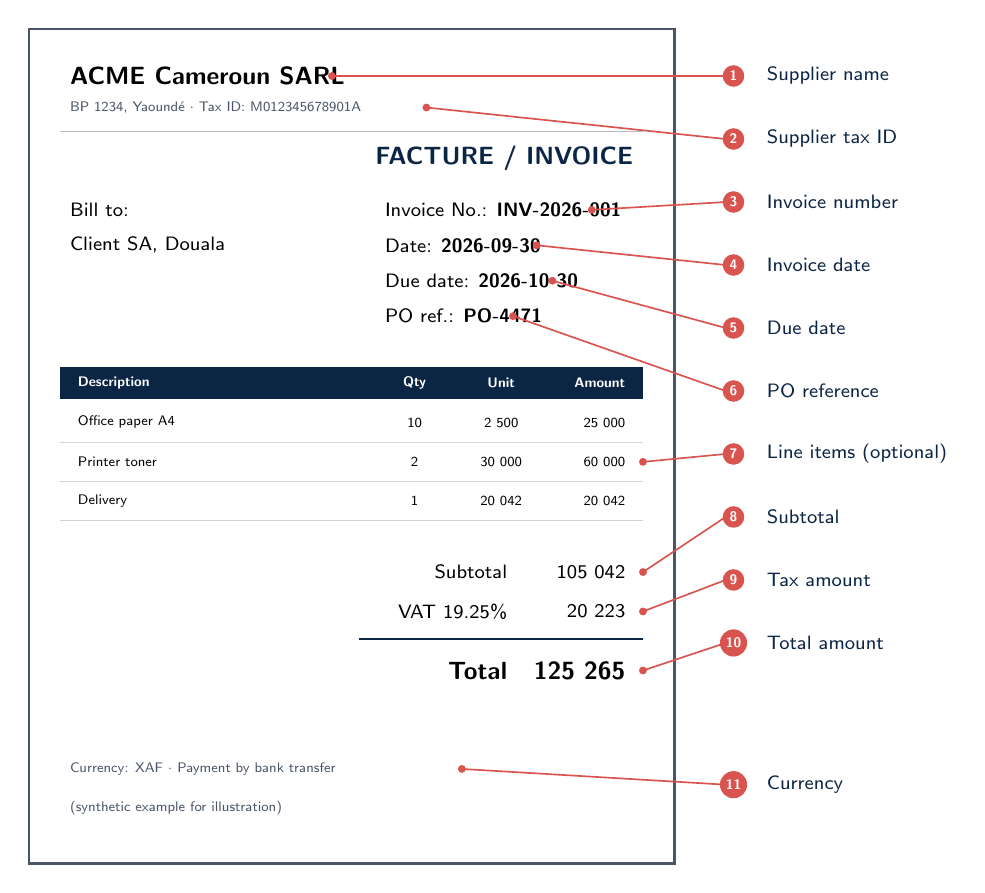
\begin{tikzpicture}[x=1cm,y=1cm]
\draw[fill=white,draw=slate,line width=0.8pt] (0,0) rectangle (8.2,10.6);
\node[font=\sffamily\bfseries\small,anchor=west] at (0.4,10.0) {ACME Cameroun SARL};
\node[font=\sffamily\tiny,text=slate,anchor=west] at (0.4,9.6) {BP 1234, Yaound\'e $\cdot$ Tax ID: M012345678901A};
\node[font=\sffamily\bfseries\small,text=navy,anchor=east] at (7.8,8.95) {FACTURE / INVOICE};
\draw[slate!40] (0.4,9.3) -- (7.8,9.3);
\node[font=\sffamily\scriptsize,anchor=west] at (0.4,8.3) {Bill to:};
\node[font=\sffamily\scriptsize,anchor=west] at (0.4,7.85) {Client SA, Douala};
\node[font=\sffamily\scriptsize,anchor=west] at (4.4,8.3) {Invoice No.: \textbf{INV-2026-001}};
\node[font=\sffamily\scriptsize,anchor=west] at (4.4,7.85) {Date: \textbf{2026-09-30}};
\node[font=\sffamily\scriptsize,anchor=west] at (4.4,7.4) {Due date: \textbf{2026-10-30}};
\node[font=\sffamily\scriptsize,anchor=west] at (4.4,6.95) {PO ref.: \textbf{PO-4471}};
\fill[navy] (0.4,5.9) rectangle (7.8,6.3);
\node[text=white,font=\sffamily\tiny\bfseries,anchor=west] at (0.5,6.1) {Description};
\node[text=white,font=\sffamily\tiny\bfseries] at (4.9,6.1) {Qty};
\node[text=white,font=\sffamily\tiny\bfseries] at (6.0,6.1) {Unit};
\node[text=white,font=\sffamily\tiny\bfseries,anchor=east] at (7.7,6.1) {Amount};
\foreach \y/\d/\q/\u/\a in {5.6/Office paper A4/10/2 500/25 000, 5.1/Printer toner/2/30 000/60 000, 4.6/Delivery/1/20 042/20 042}{
  \node[font=\sffamily\tiny,anchor=west] at (0.5,\y) {\d}; \node[font=\sffamily\tiny] at (4.9,\y) {\q}; \node[font=\sffamily\tiny] at (6.0,\y) {\u}; \node[font=\sffamily\tiny,anchor=east] at (7.7,\y) {\a};
  \draw[slate!25] (0.4,\y-0.25) -- (7.8,\y-0.25);}
\node[font=\sffamily\scriptsize,anchor=east] at (6.2,3.7) {Subtotal};  \node[font=\sffamily\scriptsize,anchor=east] at (7.7,3.7) {105 042};
\node[font=\sffamily\scriptsize,anchor=east] at (6.2,3.2) {VAT 19.25\%}; \node[font=\sffamily\scriptsize,anchor=east] at (7.7,3.2) {20 223};
\draw[navy,line width=0.8pt] (4.2,2.85) -- (7.8,2.85);
\node[font=\sffamily\small\bfseries,anchor=east] at (6.2,2.45) {Total}; \node[font=\sffamily\small\bfseries,anchor=east] at (7.7,2.45) {125 265};
\node[font=\sffamily\tiny,text=slate,anchor=west] at (0.4,1.2) {Currency: XAF $\cdot$ Payment by bank transfer};
\node[font=\sffamily\tiny,text=slate,anchor=west] at (0.4,0.7) {(synthetic example for illustration)};
% callouts: number / start x,y / label y
\foreach \n/\x/\y/\ty in {1/3.85/10.0/10.0, 2/5.05/9.6/9.2, 3/7.15/8.3/8.4, 4/6.45/7.85/7.6, 5/6.65/7.4/6.8, 6/6.15/6.95/6.0, 7/7.8/5.1/5.2, 8/7.8/3.7/4.4, 9/7.8/3.2/3.6, 10/7.8/2.45/2.8, 11/5.5/1.2/1.0}{
  \draw[coral,line width=0.6pt] (\x,\y) -- (8.85,\ty);
  \fill[coral] (\x,\y) circle (0.05);
  \node[circle,fill=coral,text=white,font=\sffamily\bfseries\tiny,inner sep=1.2pt] at (8.95,\ty) {\n};}
\foreach \n/\t/\ty in {1/Supplier name/10.0, 2/Supplier tax ID/9.2, 3/Invoice number/8.4, 4/Invoice date/7.6, 5/Due date/6.8, 6/PO reference/6.0, 7/Line items (optional)/5.2, 8/Subtotal/4.4, 9/Tax amount/3.6, 10/Total amount/2.8, 11/Currency/1.0}{
  \node[font=\sffamily\scriptsize,anchor=west,text=navy] at (9.25,\ty) {\t};}
\end{tikzpicture}
}
\caption{Anatomy of an invoice (synthetic example) with the fields to extract.}\label{fig:invoice}
\end{figure}

{\tblstart\footnotesize
\begin{longtable}{L{0.7cm}L{2.7cm}L{1.4cm}L{1.4cm}L{4.0cm}L{2.6cm}}
\hdrrow \hdr{No.} & \hdr{Field} & \hdr{Type} & \hdr{Required} & \hdr{Validation} & \hdr{Candidate ERP field}\\ \endhead
1 & Supplier name & text & Yes & Non-empty; matched to known suppliers if available. & partner\\
2 & Supplier tax ID & text & No & Pattern check where format is known. & partner VAT\\
3 & Invoice number & text & Yes & Non-empty; used in duplicate check. & vendor reference\\
4 & Invoice date & date & Yes & Parses; plausible range. & invoice date\\
5 & Due date & date & No & Not before invoice date. & due date\\
6 & PO reference & text & No & Format check if configured. & origin / purchase order\\
7 & Line items & table & No & Quantity $\times$ unit price $\approx$ amount. & invoice lines\\
8 & Subtotal & decimal & Yes & Parses with locale rules. & untaxed amount\\
9 & Tax amount & decimal & Yes & Parses; consistent with rate if known. & tax amount\\
10 & Total amount & decimal & Yes & Subtotal + tax $\approx$ total within tolerance. & total amount\\
11 & Currency & code & Yes & Known currency code or symbol; consistent. & currency\\
\hline
\end{longtable}}

\chapter{Non-Functional Requirements}
{\tblstart\small
\begin{longtable}{L{1.6cm}L{2.4cm}L{5.0cm}L{4.6cm}}
\hdrrow \hdr{ID} & \hdr{Category} & \hdr{Requirement} & \hdr{Verification}\\ \endhead
NFR-01 & Security & Authenticate users, authorise every protected action, keep secrets out of code, restrict stored files. & Access-control and file-access tests.\\
NFR-02 & Privacy & Collect only necessary data; synthetic or authorised test documents; define retention. & Data-handling checklist.\\
NFR-03 & Reliability & A failed step produces a visible, recoverable state; no silent job loss. & Failure-injection tests.\\
NFR-04 & Traceability & Stable identifiers and timestamps for documents and runs. & Inspection of records.\\
NFR-05 & Maintainability & Separate API, domain logic, OCR, validation, storage and ERP adapter. & Code structure review.\\
NFR-06 & Portability & Setup reproducible from documentation and Docker images. & Clean-machine setup test.\\
NFR-07 & Performance & Measure per-stage and end-to-end time; set targets after a baseline. & Timed runs on the test set.\\
NFR-08 & Usability & Reviewers find doubtful fields and understand errors without logs. & Task-based usability check.\\
NFR-09 & Scalability & OCR separable from interactive requests; scalable later. & Architecture review, worker test.\\
NFR-10 & Observability & Structured logs and health without sensitive content. & Log inspection.\\
\hline
\end{longtable}}

\section{Business rules}
\begin{enumerate}
\item[BR-1] No ERP submission before validation and approval by an authorised reviewer.
\item[BR-2] Low-confidence fields are always visible to the reviewer; confidence is not proof.
\item[BR-3] Likely duplicates are flagged, never deleted automatically.
\item[BR-4] ERP requests carry an idempotency key.
\item[BR-5] Corrections keep the original value, new value, actor, time and reason.
\item[BR-6] Failed integration attempts are retryable without duplicate records.
\end{enumerate}

\chapter{Use Cases}
\section{Use-case diagram}
\begin{figure}[H]\centering
\resizebox{\textwidth}{!}{\begin{tikzpicture}[x=1cm,y=1cm]
\draw[rounded corners=6pt,fill=mist,draw=navy,line width=0.8pt] (3.0,-0.4) rectangle (14.0,10.9);
\node[font=\sffamily\bfseries\small,text=navy] at (8.5,10.5) {\projname{} system};
\node[ucase,minimum width=4.4cm] (u1) at (6.6,9.3)  {Upload document};
\node[ucase,minimum width=4.4cm] (u2) at (6.6,8.0)  {Track status and search documents};
\node[ucase,minimum width=4.4cm] (u3) at (6.6,6.7)  {Review and correct fields};
\node[ucase,minimum width=4.4cm] (u4) at (6.6,5.4)  {Approve or reject record};
\node[ucase,minimum width=4.4cm] (u5) at (6.6,4.1)  {Submit approved record to ERP};
\node[ucase,minimum width=4.4cm] (u6) at (6.6,2.8)  {View audit trail and metrics};
\node[ucase,minimum width=4.4cm] (u7) at (6.6,1.5)  {Configure rules and thresholds};
\node[ucase,minimum width=4.4cm] (u8) at (6.6,0.2)  {Manage users and roles};
\node[ucase,minimum width=2.3cm,fill=sand,draw=amber!80!black] (v1) at (12.2,9.3) {Validate file};
\node[ucase,minimum width=2.3cm,fill=sand,draw=amber!80!black] (v2) at (12.2,4.1) {Validate ERP payload};
\draw[arrd] (u1) -- node[lbl,above]{\stereo{include}} (v1);
\draw[arrd] (u5) -- node[lbl,above]{\stereo{include}} (v2);
\actor{op}{1.2}{8.1}{Document\\operator}
\actor{rv}{1.2}{4.8}{Reviewer /\\accountant}
\actor{ad}{1.2}{1.0}{Administrator /\\supervisor}
\node[box,fill=blush,draw=coral,minimum width=1.9cm,minimum height=1.4cm,align=center] (erp) at (15.9,4.1) {\stereo{system}\\\textbf{ERP / Odoo}\\(or mock API)};
\foreach \a/\u in {op/u1,op/u2, rv/u2,rv/u3,rv/u4, ad/u6,ad/u7,ad/u8, rv/u6}{\draw[color=navy,line width=0.6pt] (\a) -- (\u);}
\draw[color=navy,line width=0.6pt] (erp.west) -- (14.0,4.1) -- (v2.east);
\end{tikzpicture}
}
\caption{Use cases and actors (all require sign-in).}\label{fig:uc1}
\end{figure}

\section{Detailed use-case specifications}
\subsection*{UC-01 Upload document}
{\tblstart\small
\begin{longtable}{L{3.0cm}L{10.8cm}}
Actor & Document operator\\
Preconditions & Operator is signed in and has the Operator role.\\
Main flow & 1. Operator selects a file. 2. System checks type, size and integrity. 3. System stores the original and its SHA-256. 4. System creates a document and a queued job. 5. System returns the document ID and status.\\
Alternative flows & 2a. File invalid: system refuses with a reason (400/413/415). 3a. Same hash already stored: system accepts but flags a probable duplicate.\\
Postconditions & Document exists in state QUEUED; an audit event \emph{upload} is recorded.\\
Requirements & FR-03, FR-04, FR-05, FR-06, FR-13\\
\hline
\end{longtable}}

\subsection*{UC-02 Review, correct and approve}
{\tblstart\small
\begin{longtable}{L{3.0cm}L{10.8cm}}
Actor & Reviewer\\
Preconditions & Document is in NEEDS\_REVIEW.\\
Main flow & 1. Reviewer opens the record. 2. System shows the source page beside extracted fields, doubtful ones highlighted. 3. Reviewer corrects fields and gives reasons. 4. Reviewer approves. 5. System stores corrections and decision and sets APPROVED.\\
Alternative flows & 4a. Reviewer rejects with a reason: state REJECTED. 3a. A correction breaks a validation rule: system shows the finding and blocks approval until resolved or explicitly overridden with a reason (override policy to be decided).\\
Postconditions & Audit events for each correction and the decision.\\
Requirements & FR-11, FR-12, FR-13, FR-22\\
\hline
\end{longtable}}

\subsection*{UC-03 Submit approved record to ERP}
{\tblstart\small
\begin{longtable}{L{3.0cm}L{10.8cm}}
Actor & Integration service (triggered by an authorised user or automatically after approval)\\
Preconditions & Document is APPROVED; ERP adapter configured.\\
Main flow & 1. System builds the ERP payload and an idempotency key. 2. System validates the payload. 3. System calls the ERP. 4. On success it stores the external reference and sets ERP\_SENT.\\
Alternative flows & 2a. Payload invalid: submission blocked, finding shown. 3a. ERP error or timeout: attempt recorded, state ERP\_FAILED; retry reuses the same key.\\
Postconditions & An ERPAttempt record exists for every try; no duplicate ERP record.\\
Requirements & FR-14, FR-15, FR-13\\
\hline
\end{longtable}}

\subsection*{UC-04 Manage users and thresholds}
{\tblstart\small
\begin{longtable}{L{3.0cm}L{10.8cm}}
Actor & Administrator\\
Main flow & Create or deactivate users, assign roles, adjust validation rules and review thresholds; every change is audited.\\
Requirements & FR-02, FR-17, FR-13\\
\hline
\end{longtable}}

\chapter{Data Requirements}
\section{Data the system stores}
Users and roles; documents (metadata, hash, storage key, status); processing runs; extracted fields with confidence and evidence; reviews; ERP attempts; audit events. Original files are stored outside the database in protected storage.

\section{Dataset requirements for OCR (Phase 8 preparation)}
\begin{itemize}
\item \textbf{Sources:} synthetic invoices generated from templates (with varied fonts, layouts and noise), invoices created by the student, and authorised real samples with personal data removed. Do not use real customer data without permission.
\item \textbf{Languages:} French and English, including accented characters, currency symbols and typical French number formats.
\item \textbf{Labels:} verified transcriptions of text lines and field-level ground truth for the test set.
\item \textbf{Split:} training, validation and test sets separated by source document or template, so the test set is truly unseen.
\item \textbf{Documentation:} dataset version, size, language mix, labelling method and known limitations.
\item \textbf{Size:} not fixed in advance; decide after the baseline shows the error level. [Decision needed with supervisor]
\end{itemize}

\section{Ethics and data handling}
Documents may contain personal and financial information. Use synthetic or anonymised data for development, restrict access, define retention, and do not send documents to external OCR services without understanding the privacy implications.

\chapter{Constraints, Assumptions and Dependencies}
\section{Constraints}
\begin{itemize}
\item One student developer and a fixed academic calendar.
\item Limited training hardware; a GPU may need a cloud notebook.
\item The ERP interface may be unavailable; a mock ERP is the fallback.
\item The jury expects measured results and a working demonstration.
\end{itemize}
\section{Assumptions}
\begin{itemize}
\item Python 3.13 and MySQL 8 can be installed on the development machine.
\item Enough invoices (real, synthetic or both) can be assembled for training and testing.
\item The supervisor approves the invoice-only scope.
\end{itemize}
\section{Dependencies}
Supervisor approval of scope; access to an ERP sandbox or Odoo instance (Phase 12); dataset availability (Phase 8); GPU or cloud access (Phase 8).

\chapter{Risk Analysis}
\begin{figure}[H]\centering
\resizebox{0.72\textwidth}{!}{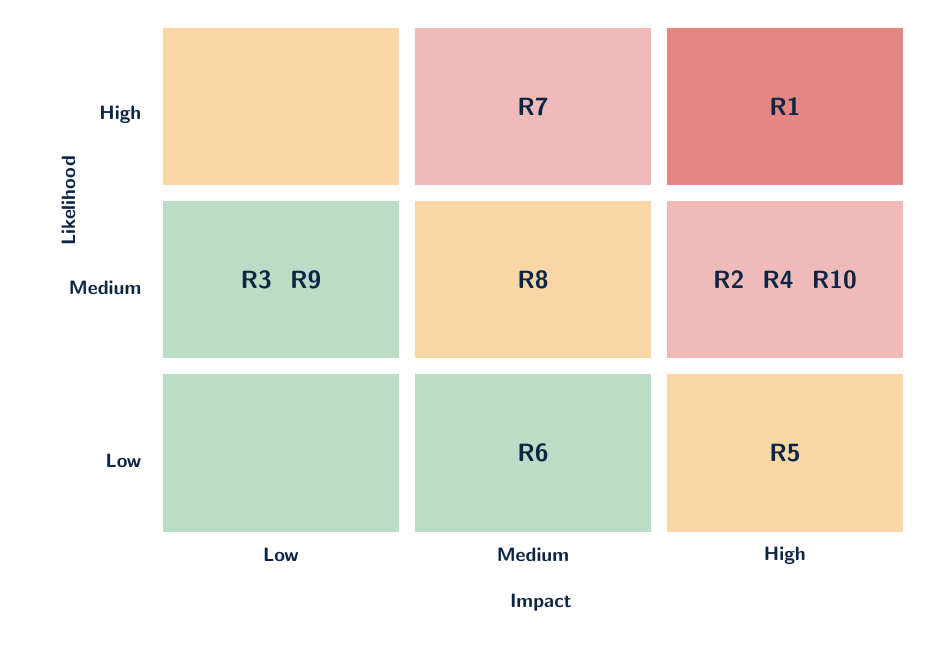
\begin{tikzpicture}[x=1cm,y=1cm]
\foreach \r/\ry in {0/High,1/Medium,2/Low}{
  \node[font=\sffamily\scriptsize\bfseries,text=navy,anchor=east] at (-0.15,{2.5-\r*2.2}) {\ry};}
\foreach \c/\cx in {0/Low,1/Medium,2/High}{
  \node[font=\sffamily\scriptsize\bfseries,text=navy] at ({1.5+\c*3.2},-3.1) {\cx};}
% cells (row 0 = high likelihood)
\foreach \r/\c/\col in {0/0/amber!45,0/1/coral!40,0/2/coral!70, 1/0/leaf!35,1/1/amber!45,1/2/coral!40, 2/0/leaf!35,2/1/leaf!35,2/2/amber!45}{
  \fill[\col] ({\c*3.2},{3.6-\r*2.2}) rectangle ({\c*3.2+3.0},{3.6-\r*2.2-2.0});}
\node[font=\sffamily\small\bfseries,text=navy] at (-1.6,2.5) {};
\node[rotate=90,font=\sffamily\scriptsize\bfseries,text=navy] at (-1.2,1.4) {Likelihood};
\node[font=\sffamily\scriptsize\bfseries,text=navy] at (4.8,-3.7) {Impact};
\node[font=\sffamily\small\bfseries,text=navy,align=center] at (7.9,2.6) {R1};  % high L, high I
\node[font=\sffamily\small\bfseries,text=navy,align=center] at (4.7,2.6) {R7};  % high L, medium I
\node[font=\sffamily\small\bfseries,text=navy,align=center] at (7.9,0.4) {R2 \ R4 \ R10}; % medium L, high I
\node[font=\sffamily\small\bfseries,text=navy,align=center] at (4.7,0.4) {R8};  % medium L, medium I
\node[font=\sffamily\small\bfseries,text=navy,align=center] at (1.5,0.4) {R3 \ R9}; % medium L, low I
\node[font=\sffamily\small\bfseries,text=navy,align=center] at (7.9,-1.8) {R5};  % low L, high I
\node[font=\sffamily\small\bfseries,text=navy,align=center] at (4.7,-1.8) {R6};  % low L, medium I
\end{tikzpicture}
}
\caption{Initial risk matrix. Identifiers refer to the table below.}\label{fig:risk1}
\end{figure}
{\tblstart\small
\begin{longtable}{L{0.9cm}L{3.4cm}L{2.0cm}L{2.0cm}L{5.0cm}}
\hdrrow \hdr{ID} & \hdr{Risk} & \hdr{Likelihood} & \hdr{Impact} & \hdr{Mitigation}\\ \endhead
R1 & Not enough labelled data & High & High & Synthetic data, templates, invoice-only scope.\\
R2 & Custom OCR under-performs & Medium & High & Baseline comparison, error analysis, replaceable OCR interface.\\
R3 & Package incompatibility & Medium & Low & Python 3.13, pinned versions.\\
R4 & ERP API unknown / no Odoo access & Medium & High & Mock ERP and adapter interface; ask for access early.\\
R5 & Sensitive data exposure & Low & High & Synthetic data, private storage, minimal logging.\\
R6 & Duplicate ERP records & Low & Medium & Idempotency keys and retry tests.\\
R7 & Scope creep & High & Medium & Written scope; extras go to future work.\\
R8 & Microservice overhead & Medium & Medium & Modular monolith first.\\
R9 & OCR job crashes & Medium & Low & Persisted status, bounded retries.\\
R10 & Training hardware or time lacking & Medium & High & Small model, cloud GPU, smaller dataset.\\
\hline
\end{longtable}}

\chapter{Project Plan}
\section{Phases and stages}
The project has 18 phases in four stages: A Foundation (1--5), B Intelligence (6--10), C Application (11--13), D Delivery (14--18). The rule is to complete one end-to-end workflow before adding architectural complexity.

\section{Proposed timeline}
\begin{warnbox}[Assumption]
The 30-week timeline is a \emph{proposal}. The real start date, deadline and supervisor checkpoints are not known and must replace these weeks.
\end{warnbox}
\begin{figure}[H]\centering
\resizebox{\textwidth}{!}{\begin{ganttchart}[x unit=0.37cm,y unit title=0.5cm,y unit chart=0.46cm,
  hgrid,hgrid style/.style={dotted,slate!40},vgrid={*{4}{draw=none},dotted},vgrid style/.style={slate!40},
  title label font=\sffamily\tiny,bar label font=\sffamily\scriptsize,bar height=0.6,
  bar/.append style={draw=none},
  canvas/.append style={draw=slate!40},
  bar label node/.append style={anchor=east,text width=4.4cm,align=right,font=\sffamily\scriptsize}]{1}{30}
\gantttitle{Proposed project weeks (assumption -- adjust to your academic calendar)}{30}\\
\gantttitlelist{1,...,30}{1}\\
\ganttbar[bar/.append style={fill=teal}]{P1 Requirements and planning}{1}{2}\\
\ganttbar[bar/.append style={fill=teal}]{P2 Design and architecture}{2}{4}\\
\ganttbar[bar/.append style={fill=teal}]{P3 Environment setup}{3}{4}\\
\ganttbar[bar/.append style={fill=teal}]{P4 Database and backend}{4}{7}\\
\ganttbar[bar/.append style={fill=teal}]{P5 Upload and storage}{7}{9}\\
\ganttbar[bar/.append style={fill=amber}]{P6 Image preprocessing}{9}{11}\\
\ganttbar[bar/.append style={fill=amber}]{P7 Baseline OCR}{10}{12}\\
\ganttbar[bar/.append style={fill=amber}]{P8 Custom OCR model}{11}{19}\\
\ganttbar[bar/.append style={fill=amber}]{P9 Information extraction}{13}{16}\\
\ganttbar[bar/.append style={fill=amber}]{P10 Validation + confidence}{16}{18}\\
\ganttbar[bar/.append style={fill=violet}]{P11 Human review}{18}{21}\\
\ganttbar[bar/.append style={fill=violet}]{P12 ERP integration}{20}{23}\\
\ganttbar[bar/.append style={fill=violet}]{P13 React web dashboard}{14}{24}\\
\ganttbar[bar/.append style={fill=coral}]{P14 Testing and evaluation}{22}{26}\\
\ganttbar[bar/.append style={fill=coral}]{P15 Security + reliability}{24}{26}\\
\ganttbar[bar/.append style={fill=coral}]{P16 Docker + deployment}{25}{27}\\
\ganttbar[bar/.append style={fill=coral}]{P17 Services + scaling (optional)}{27}{29}\\
\ganttbar[bar/.append style={fill=coral}]{P18 Report and defence}{24}{30}
\end{ganttchart}
}
\caption{Proposed Gantt chart (colours: teal = foundation, amber = intelligence, violet = application, red = delivery).}\label{fig:gantt}
\end{figure}

\section{Milestones}
{\tblstart\small
\begin{longtable}{L{1.2cm}L{6.2cm}L{3.0cm}L{3.2cm}}
\hdrrow \hdr{ID} & \hdr{Milestone} & \hdr{Proposed week} & \hdr{Evidence}\\ \endhead
M1 & Requirements approved by supervisor & 2 & Signed Phase 1 document\\
M2 & Backend + database + upload working & 9 & Passing tests, demo\\
M3 & Baseline OCR results & 12 & CER/WER table\\
M4 & Custom OCR trained and compared & 19 & Evaluation report\\
M5 & End-to-end workflow with mock ERP & 23 & Recorded demo run\\
M6 & Evaluation and security complete & 26 & Test reports\\
M7 & Deployed system and final report & 30 & Report, slides, demo\\
\hline
\end{longtable}}

\section{Definition of done}
A phase is done when: its deliverable exists, automated tests for it pass, documentation is updated, and the result is demonstrable to the supervisor.

\chapter{Traceability Matrix}
Each objective is linked to requirements and to the test that will prove it.
{\tblstart\small
\begin{longtable}{L{1.0cm}L{5.0cm}L{4.4cm}L{3.2cm}}
\hdrrow \hdr{Obj.} & \hdr{Requirements} & \hdr{Verified by} & \hdr{Phase}\\ \endhead
O1 & FR-03, 04, 05, 06 & API and upload tests & 5, 14\\
O2 & FR-07 & Preprocessing A/B comparison & 6\\
O3 & FR-08, NFR-07 & CER/WER experiment & 7, 8\\
O4 & FR-09 & Field-level F1 evaluation & 9\\
O5 & FR-11, FR-17 & Review-routing evaluation & 10\\
O6 & FR-10 & Seeded-error unit tests & 10\\
O7 & FR-12, 16, 19, 22, NFR-08 & Usability check, UI tests & 11, 13\\
O8 & FR-13, NFR-04 & Audit-log tests & 4, 11\\
O9 & FR-14, 15, 20, 21 & Mock-ERP integration tests & 12\\
O10 & NFR-06, NFR-09, NFR-10, FR-18 & Clean-machine setup, health checks & 16, 17\\
\hline
\end{longtable}}

\chapter{Open Decisions and Sign-off}\label{sec:decisions}
\section{Decisions needed to close Phase 1}
{\tblstart\small
\begin{longtable}{L{0.9cm}L{6.0cm}L{4.4cm}L{2.5cm}}
\hdrrow \hdr{No.} & \hdr{Decision} & \hdr{Current proposal} & \hdr{Owner}\\ \endhead
D1 & Final project name & \projname{} (working name) & Student\\
D2 & Supervisor name and checkpoints & To be completed & Student / supervisor\\
D3 & Prototype document type & Invoices only & Supervisor\\
D4 & ERP target & Mock ERP first, Odoo later & Student / supervisor\\
D5 & Odoo version and access & Unknown & Student\\
D6 & Dataset source and size & Synthetic + authorised samples; size after baseline & Student / supervisor\\
D7 & Training hardware & Local GPU or cloud notebook & Student\\
D8 & Real calendar and deadlines & Replace proposed 30 weeks & Student\\
D9 & Policy when a reviewer overrides a validation error & Allow with mandatory reason & Supervisor\\
\hline
\end{longtable}}

\section{Phase 1 completion checklist}
\begin{itemize}
\item[\fbox{\rule{0pt}{6pt}\rule{6pt}{0pt}}] Problem, objectives and scope reviewed with the supervisor.
\item[\fbox{\rule{0pt}{6pt}\rule{6pt}{0pt}}] Decisions D1--D9 answered.
\item[\fbox{\rule{0pt}{6pt}\rule{6pt}{0pt}}] Functional and non-functional requirements accepted.
\item[\fbox{\rule{0pt}{6pt}\rule{6pt}{0pt}}] Provisional targets agreed as planning values.
\item[\fbox{\rule{0pt}{6pt}\rule{6pt}{0pt}}] Timeline replaced by the real academic calendar.
\item[\fbox{\rule{0pt}{6pt}\rule{6pt}{0pt}}] Cover page completed.
\end{itemize}

\section{Approval}
\tblstart\small
\begin{tabular}{L{4.2cm}L{4.5cm}L{3.2cm}}
\hline
Student & \studentname & Date:\\[0.6cm]
\hline
Supervisor & \supervisorname & Date:\\[0.6cm]
\hline
\end{tabular}


\end{document}
